\subsection{Просмотр списка диалогов}
\label{sec:usage:dialogues}

После разблокировки клиента, пользователь попадает в главный экран приложения, который показывает список диалогов, рисунок \ref{sec:usage:dialogues:ui} А. В список диалогов попадают все диалоги, которые имеют хотя бы одно сообщение. Диалоги сортируются по дате последнего сообщения, открыть конкретный диалог можно нажав на ячейку с его последним сообщением в таблице. Для удаления диалога, нужно потянуть ячейку диалога влево и нажать кнопку <<Удалить>>.

\subsection{Просмотр сообщений диалога и отправка сообщения}
\label{sec:usage:dialogue}

После выбора диалога, пользователь попадает в экран списка сообщений конкретного диалога, рисунок \ref{sec:usage:dialogues:ui} Б. На экране выводится список сообщений, отсортированный в хронологическом порядке. У каждого сообщения есть статус, который представлен в пользовательском интерфейсе в виде кружка в правом нижнем углу ячейки сообщения. В таблице \ref{table:usage:dialogues:statusdesc} представлены возможные варианты статуса сообщения и соответствующее им состояния интерфейса.

\begin{itemize}
	\item отправляется;
	\item доставлено;
	\item прочитано.
\end{itemize}

Для отправки сообщения, пользователь должен ввести текст в поле <<Сообщение>> и нажать кнопку <<Отправить>>.

\begin{figure}[h]
  \centering
    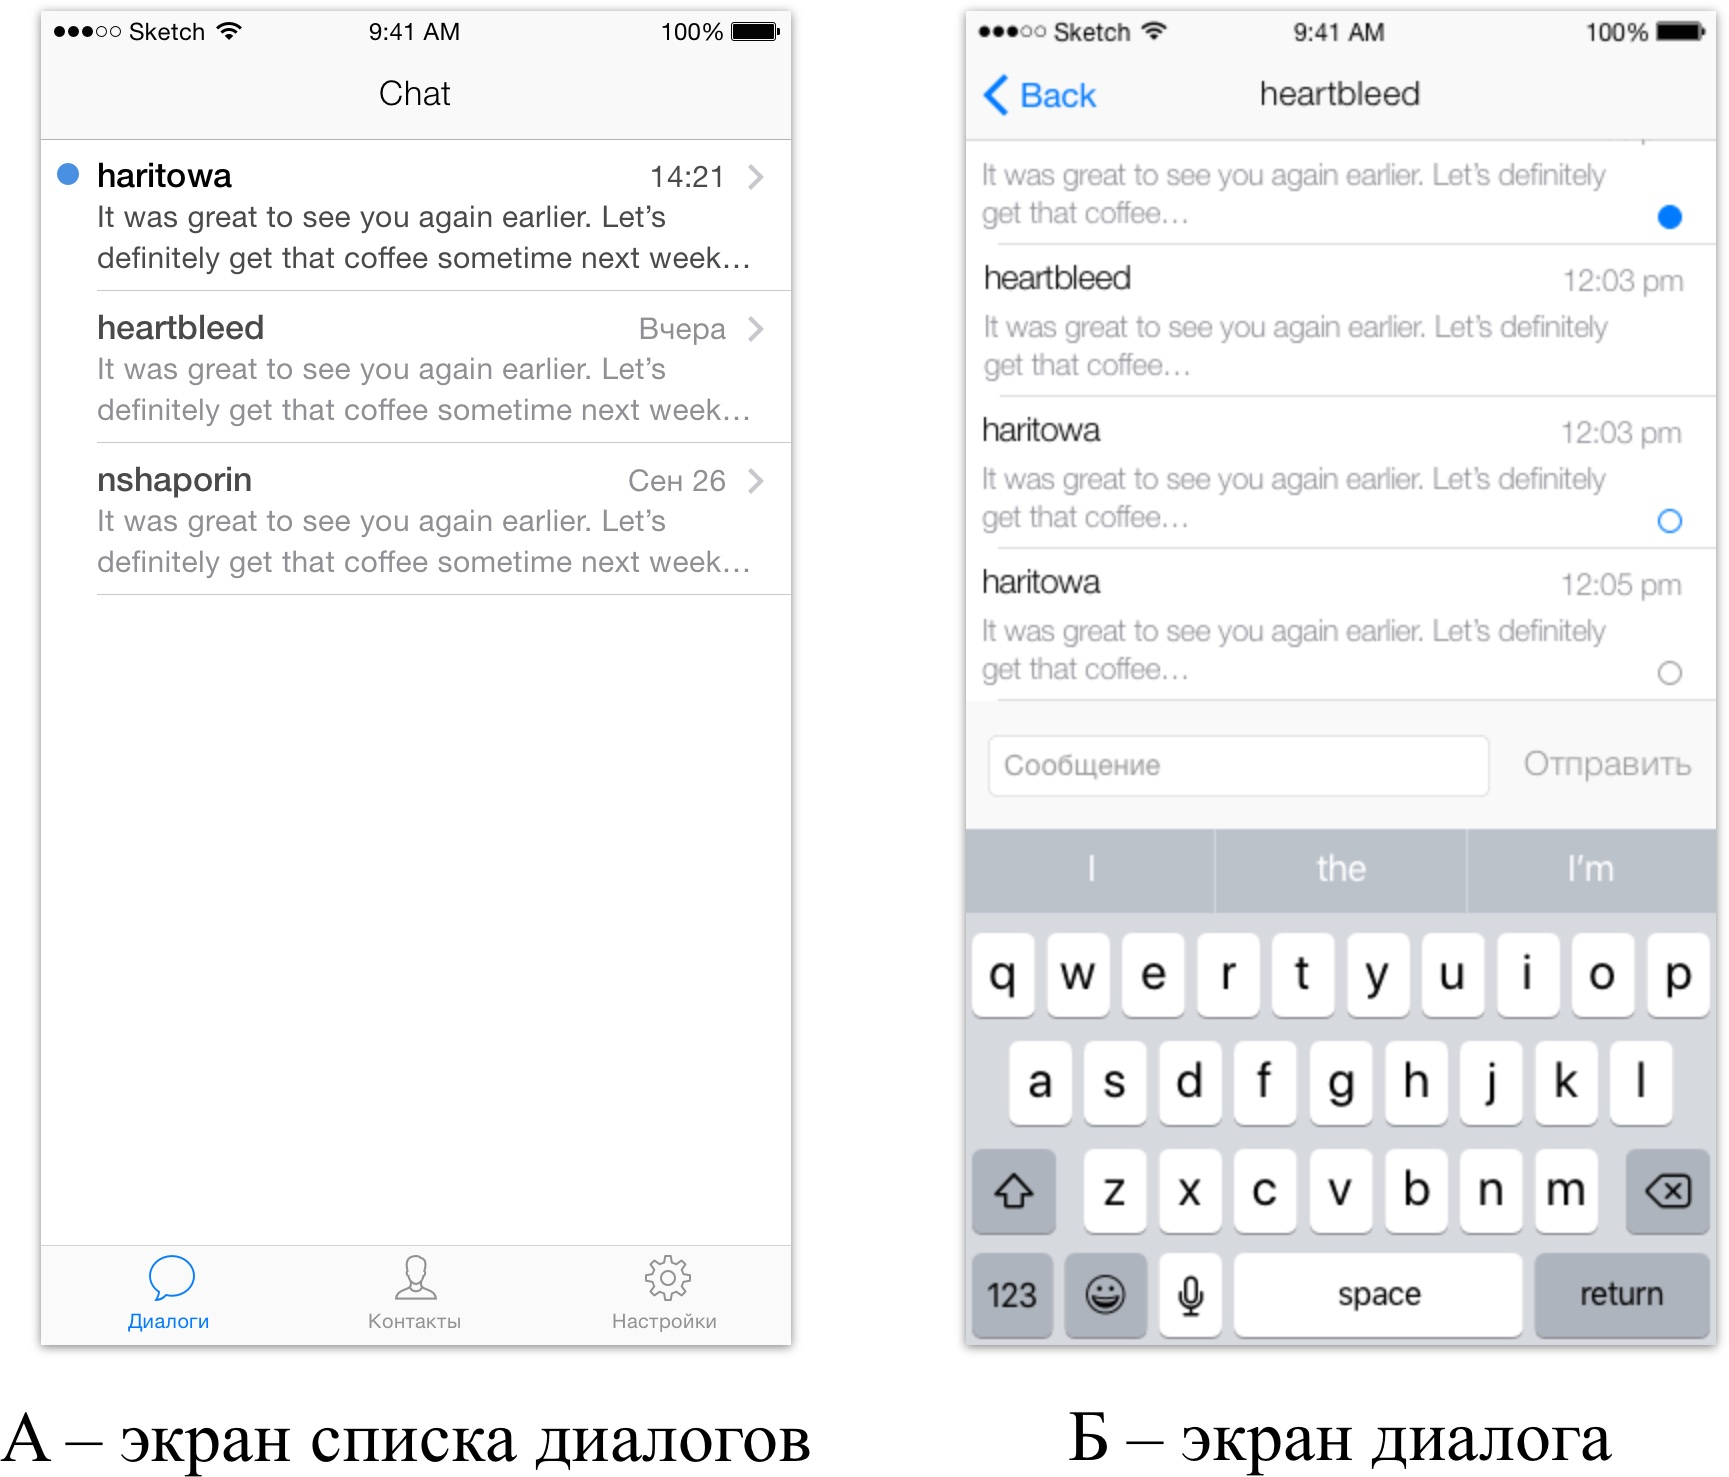
\includegraphics[width=0.75\textwidth]{inc/img/ui/dialogue.jpg}
  \caption{Экраны диалога и списка диалогов}
  \label{sec:usage:dialogues:ui}
\end{figure}

\begin{table}[!ht]
  \caption{Описание статусов сообщения}
  \label{table:usage:dialogues:statusdesc}
  \centering
  \begin{tabularx}{\linewidth}{
    |>{\centering\hsize=0.75\hsize}X|
    >{\centering\hsize=1\hsize}X|
    >{\centering\arraybackslash\hsize=1.25\hsize}X|
  }
	\hline
	Название статуса & Описание статуса & Описание интерфейса \\

	\hline
	Отправляется & Сообщение отправляется на сервер & Круг с белой заливкой и серой рамкой \\

	\hline
	Отправлено & Сообщение отправлено на сервер & Круг с белой заливкой и синей рамкой \\

	\hline
	Прочитано & Сообщение прочитано получателем & Круг с синей заливкой или отсутствие круга, если после текущего сообщения есть другие прочитанные \\

	\hline
  \end{tabularx}
\end{table}

Как можно заметить из всего раздела \ref{sec:usage}, при разработке приложения происходил постоянный процесс поиска сбалансированного решения, предоставляющего высокий уровень безопасности при передачи и хранении данных и не наносящий значительного сокращения качества пользовательского опыта.